% !TEX program = xelatex
\documentclass[14pt,a4paper,oneside]{extbook}

\usepackage{kieu_bao_cao}

\newacronym{UAV}{UAV}{unmanned aerial vehicle}
\newacronym{VTOL}{VTOL}{vertical take-off and landing}
\newacronym{rpm}{rpm}{revolutions per minute}
\newacronym{BLDC}{BLDC}{brushless DC}
\newacronym{ESC}{ESC}{electronic speed controller}
\newacronym{LiPo}{LiPo}{lithium polymer}
\newacronym{FCU}{FCU}{flight control unit}
\newacronym{PWM}{PWM}{pulse-width modulation}
\newacronym{DC}{DC}{direct current}


\begin{document}

\singlespacing

\begin{titlepage}
\thispagestyle{empty}
\begin{tikzpicture}[remember picture,overlay]
    \node[inner sep=0pt] at (current page.center) {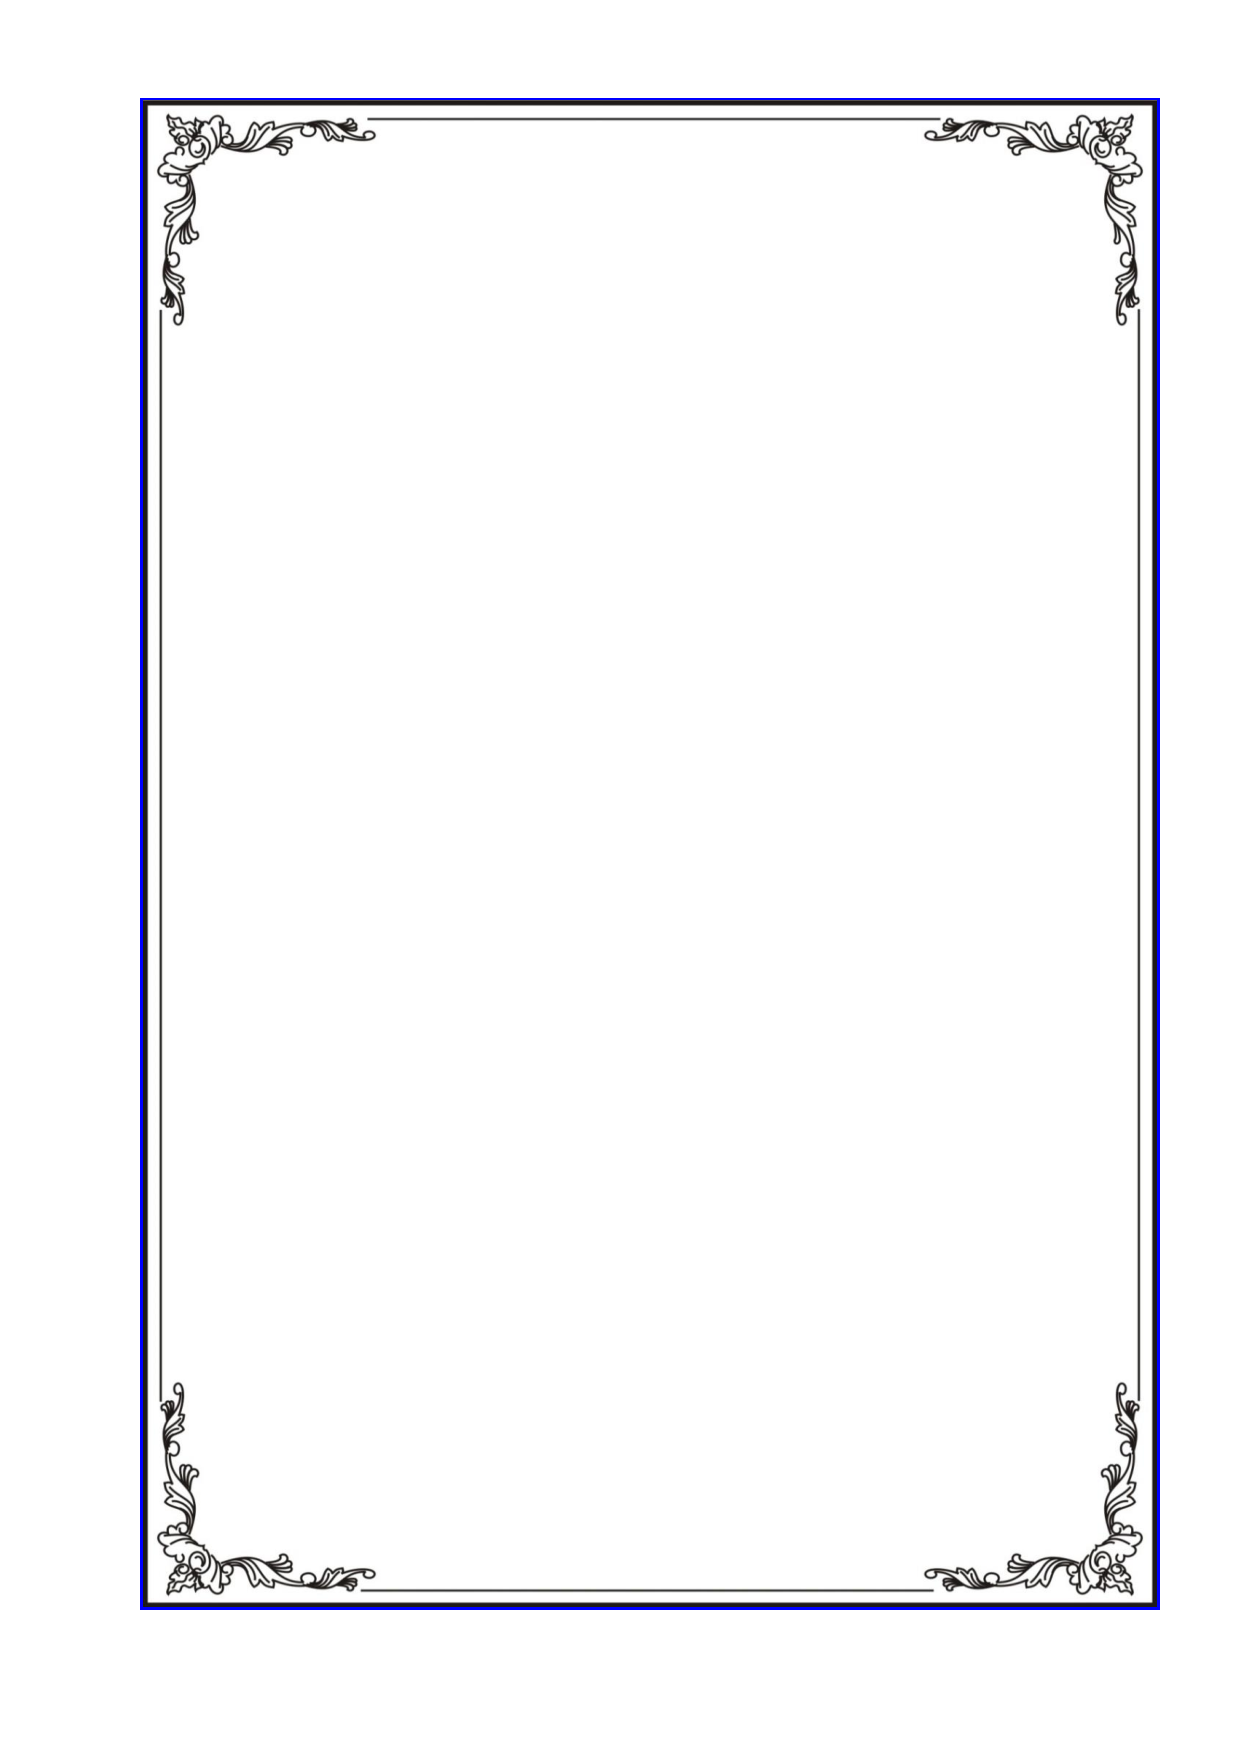
\includegraphics[width=\paperwidth,height=\paperheight]{Figures/title page cover.pdf}};
    \node[anchor=south] at ([yshift=3.0cm]current page.south) {\large\itshape Hà Nội -- 2025};
\end{tikzpicture}

\begin{center}
\vspace*{-0.7cm}
{\large\bfseries BỘ CÔNG THƯƠNG\par}
{\large\bfseries TRƯỜNG ĐẠI HỌC CÔNG NGHIỆP HÀ NỘI\par}
{\large\bfseries TRƯỜNG CƠ KHÍ -- Ô TÔ\par}
{\large\bfseries KHOA CƠ ĐIỆN TỬ\par}

\vspace{1.0cm}


\includegraphics[width=2.8cm]{Figures/HaUI_logo.jpg}

\vspace{1.0cm}

{\fontsize{26}{28}\bfseries\color{red}ĐỒ ÁN TỐT NGHIỆP\par}
\vspace{0.15cm}
{\Large\bfseries ĐẠI HỌC\par}
\vspace{0.8cm}

{\large\bfseries NGÀNH: ROBOT VÀ TRÍ TUỆ NHÂN TẠO\par}
\vspace{0.4cm}
{\Large\bfseries ĐỀ TÀI:\par}
\vspace{0.15cm}
{\normalsize\bfseries NGHIÊN CỨU, THIẾT KẾ, CHẾ TẠO HỆ THỐNG KIỂM TRA LINH KIỆN MẠCH ĐIỆN TỬ SỬ DỤNG TAY MÁY ROBOT KẾT HỢP PLC VÀ XỬ LÝ ẢNH\par}

\vspace{1.3cm}

\begin{tabular}{@{}p{6.5cm}>{\raggedright\arraybackslash}p{7.5cm}@{}}
\textbf{Giáo viên hướng dẫn:} & ThS. Bùi Huy Anh \\
\textbf{Nhóm sinh viên thực hiện:} & Nguyễn Văn Hưng \\
& Vũ Trọng Lộc \\
& Chu Quang Tiến \\
\end{tabular}
\end{center}
\end{titlepage}


\pagenumbering{Roman}

%%%%%%%%%%%%%%%% Tóm tắt và lời cảm ơn %%%%%%%%%%%%%%%
\onehalfspacing
\newcommand{\AbstractName}{MỞ ĐẦU}
\chapter*{\AbstractName}
\addcontentsline{toc}{chapter}{\AbstractName}

Kính gửi Thầy/Cô,

Em xin gửi lời cảm ơn sâu sắc tới Thầy ThS. Bùi Huy Anh và thầy Phạm Tiến Hùng cùng toàn thể các Thầy, Cô trong Khoa Cơ điện tử đã tận tình hướng dẫn và hỗ trợ em trong suốt quá trình thực hiện đồ án tốt nghiệp. Nhờ sự quan tâm, chỉ bảo tận tụy của Thầy, em đã có thể hoàn thành đồ án một cách hiệu quả và đạt được kết quả đúng như kỳ vọng. 

Em thật sự biết ơn sự đồng hành của Thầy không chỉ về mặt chuyên môn mà còn cả tinh thần. Những lời chỉ dẫn tận tâm, các góp ý quý báu của Thầy đã giúp em nhìn nhận vấn đề một cách toàn diện hơn, từ đó xây dựng nội dung đồ án một cách logic, rõ ràng và hoàn chỉnh hơn. 

Em hiểu rằng Thầy luôn có rất nhiều công việc và trách nhiệm, nhưng vẫn dành thời gian để theo sát, hỗ trợ em trong từng giai đoạn của quá trình làm đồ án. Em trân trọng sự cống hiến đó và xin bày tỏ lòng biết ơn chân thành. 

Mặc dù đã nỗ lực hết mình, nhưng do hạn chế về kinh nghiệm thực tế và kiến thức còn chưa sâu rộng, bài báo cáo của em chắc chắn vẫn còn nhiều thiếu sót. Em rất mong nhận được những góp ý từ Thầy/Cô để có thể cải thiện và hoàn thiện bản thân hơn nữa trong tương lai.

Trân trọng cảm ơn!
\singlespacing

%%%%%%%%%%%%%%%% Tóm tắt và lời cảm ơn end %%%%%%%%%%%%%%


%%%%%%%%%%%%%%%% Danh sách hình ảnh, bảng, thuật ngữ %%%%%%%%%%%%%%%

{\sloppy
\tableofcontents % chèn mục lục
\listoffigures % chèn danh sách hình ảnh
\listoftables % chèn danh sách bảng
}

\renewcommand{\acronymname}{DANH MỤC KÝ HIỆU, CHỮ VIẾT TẮT}
\addcontentsline{toc}{chapter}{DANH MỤC KÝ HIỆU, CHỮ VIẾT TẮT}
\printglossary[type=\acronymtype, nonumberlist]
%%%%%%%%%%%%%%%% Danh sách hình ảnh, bảng, thuật ngữ end %%%%%%%%%%%%%%

\cleardoublepage
\pagenumbering{arabic}
\setcounter{page}{1}
\onehalfspacing

%%%%%%%%%%%%%%%% Nội dung chính %%%%%%%%%%%%%%%%%%%%%%%%
\chapter{GIỚI THIỆU CHUNG} \label{chap:intro}

Chương này trình bày về tổng quan

\section{Lịch sử nghiên cứu}

\begin{figure}[ht]
      \centering
      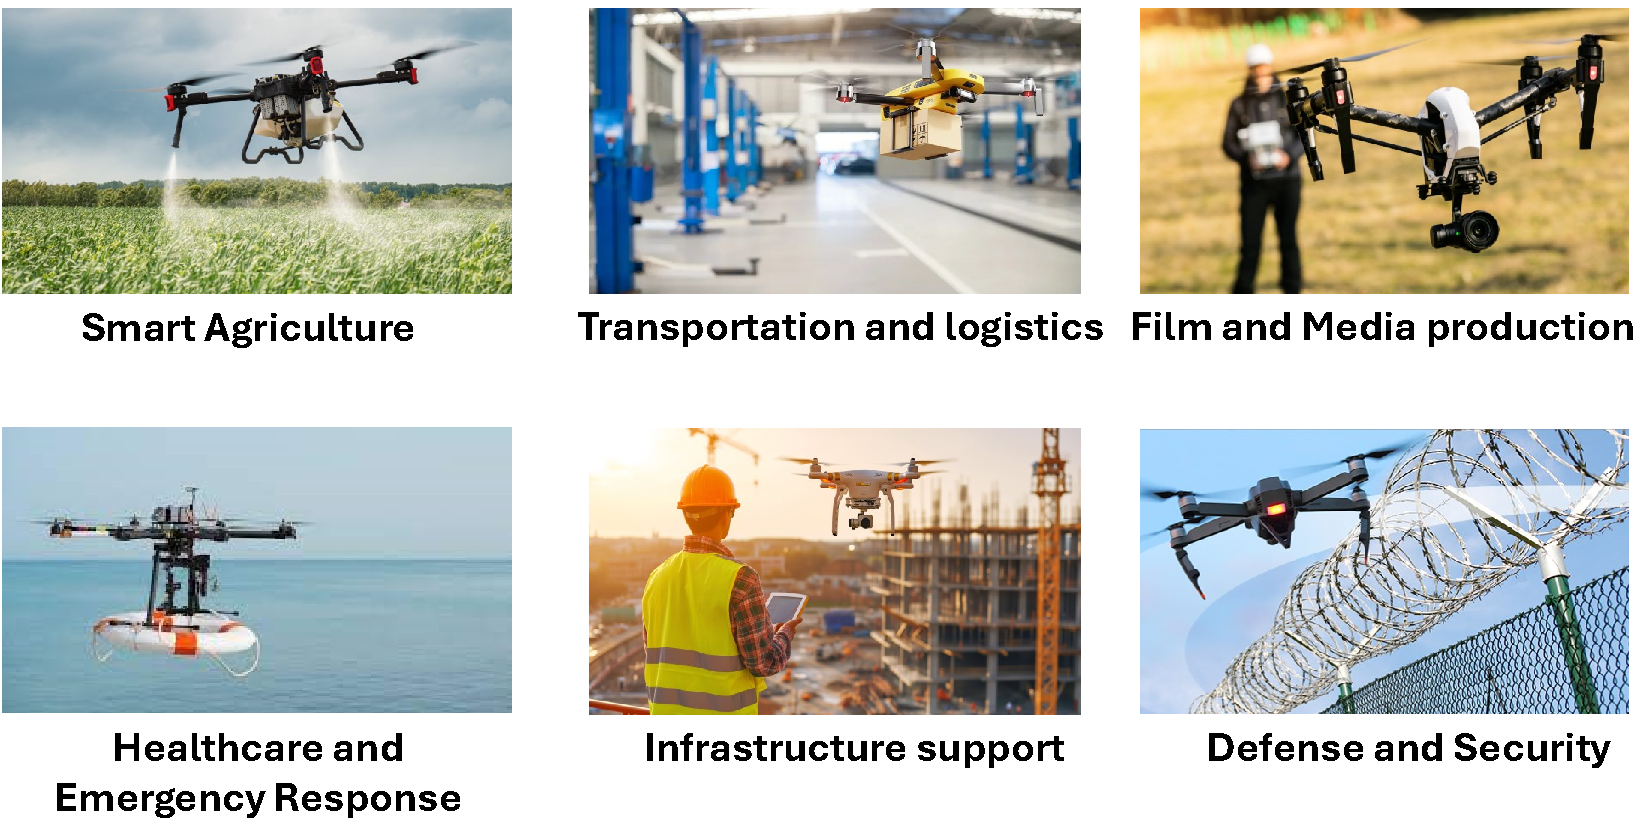
\includegraphics[scale=0.53]{Figures/drone application.pdf}
      \caption{Ứng dụng công nghệ robot trong sản xuất}
      \label{fig: drone application}
\end{figure}

Trong bối cảnh công nghiệp 4.0 đang phát triển mạnh mẽ, việc tự động hóa các khâu sản xuất và kiểm tra sản phẩm trong ngành điện – điện tử ngày càng được quan tâm. Trước đây, việc kiểm tra linh kiện mạch điện tử chủ yếu được thực hiện thủ công bởi con người, phụ thuộc vào kinh nghiệm và độ chính xác của kỹ thuật viên. Tuy nhiên, phương pháp này tốn nhiều thời gian, dễ sai sót và khó đáp ứng yêu cầu sản xuất hàng loạt với độ chính xác cao. Chính vì vậy, các hướng nghiên cứu về tự động hóa kiểm tra linh kiện đã được hình thành từ sớm, đặc biệt là trong lĩnh vực robot công nghiệp và xử lý ảnh máy tính.

Từ những năm 1990, các robot công nghiệp đã được sử dụng rộng rãi trong dây chuyền sản xuất linh kiện điện tử tại Nhật Bản, Hàn Quốc và Đức. Ban đầu, robot chủ yếu đảm nhiệm thao tác gắp – đặt linh kiện (pick and place) với độ chính xác cao, nhưng khả năng “nhận biết” linh kiện vẫn còn hạn chế do chưa có sự kết hợp với thị giác máy tính. Đến giai đoạn 2010 trở lại đây, cùng với sự phát triển của camera công nghiệp, thị giác máy tính (computer vision) và trí tuệ nhân tạo (AI), các hệ thống robot đã được nâng cấp để có thể phát hiện, nhận dạng và phân loại linh kiện một cách tự động.


\section{Đối tượng và phạm vi nghiên cứu}

\subsection{Đối tượng nghiên cứu}

Đối tượng mà đề tài nhóm tập trung nghiên cứu là mạch nguồn ổn áp tuyến tính, trong đó xem xét hai trạng thái chính: mạch đã lắp đầy đủ linh kiện và mạch bị thiếu một hoặc nhiều linh kiện. Việc lựa chọn lỗi thiếu linh kiện làm trọng tâm là do đây là dạng lỗi thường xảy ra trong quá trình sản xuất và có thể ảnh hưởng nghiêm trọng đến hoạt động ổn định của thiết bị. Thông qua hệ thống sử dụng camera và xử lý ảnh, kết hợp với tay máy robot và PLC, hình ảnh của các bo mạch sẽ được thu thập, phân tích và phân loại nhằm phát hiện sự thiếu hụt linh kiện. Mục tiêu là xây dựng một hệ thống kiểm tra tự động, có khả năng phát hiện lỗi thiếu linh kiện trên mạch nguồn ổn áp tuyến tính với độ chính xác cao, từ đó nâng cao hiệu quả kiểm tra và đảm bảo chất lượng sản phẩm đầu ra.

\section{Cấu trúc báo cáo}

Bài báo cáo bao gồm các nội dung sau:

\begin{itemize}
    \item Chương \hyperref[chap:intro]{1} Giới thiệu chung về các nội dung liên quan đến đề tài.

    \item Chương \hyperref[chap:background]{2} cơ sở lý thuyết để giới thiệu các thiết bị sử dụng trong mô hình.

    \item Chương \hyperref[chap:tombo-L1]{3} tính toán, thiết kế và chế tạo.

    \item Chương \hyperref[chap:tombo-encoder]{4} chế tạo mô hình và đánh giá.

    \item Chương \hyperref[chap:conclusion]{5} tổng kết và hướng nghiên cứu tương lai.
\end{itemize}

\chapter{CƠ SỞ LÝ THUYẾT} \label{chap:background}

This chapter presents a structured review of key techniques that enhance quadrotor safety and resilience during flight. It is organized into three main sections. The first section introduces collision avoidance strategies based on vision and perception, focusing on how drones detect and react to nearby obstacles in advance. The second section explores advanced control methods, with an emphasis on the $\mathcal{L}_1$Quad approach, which enables the quadrotor to maintain stability and adapt to external disturbances such as collisions or deformation of Tombo propellers. The final section discusses sensor-based collision detection, highlighting methods that utilize onboard sensors and passive mechanical responses to identify and localize collision events in real time.

\section{Collision Avoidance strategies}
Numerous collision avoidance strategies have been developed for \gls{UAV}s to ensure safe navigation, especially in cluttered or dynamic environments. These methods typically fall into categories such as geometric planning, force-field approaches, optimization-based schemes, and sense-and-avoid systems~\cite{avoidancetypes,avoidancetypes2}. Central to these strategies is integrating onboard sensors that perceive the environment and guide the \gls{UAV}’s response.

Vision-based sensors are widely adopted due to their rich spatial sensing capabilities and low payload weight. Among these, monocular vision offers the simplest hardware setup, relying on a single camera to extract visual features from sequential images. While machine learning methods such as YOLO-based detectors or neural networks~\cite{YoloFastest} can improve detection accuracy, they often require significant onboard computational power. Simpler alternatives include image processing approaches that identify color or shape-defined objects~\cite{monocolor}, but they struggle with unknown or unstructured obstacles. 

In~\cite{monocularcamera}, monocular vision was used for tasks such as landing on moving platforms. However, it remains insufficient for detecting large or static obstacles like buildings. To address this, stereo vision systems are employed to generate disparity maps for depth estimation. For instance,~\cite{avoidancetypes} developed a biologically inspired stereo system mounted on a servo, allowing owl-like head movements to track dynamic obstacles. Another approach, "pushbroom stereo," combines stereo imagery with forward motion and lightweight processing for fast obstacle detection~\cite{pushbroom}.
\chapter{TÍNH TOÁN, THIẾT KẾ VÀ CHẾ TẠO HỆ THỐNG}
\label{chap:tombo-L1}

This chapter focuses on the application of the $\mathcal{L}_1$Quad controller to the Tombo quadrotor, enabling effective handling of mild and short-duration collisions occurring while the drone follows a predefined trajectory towards a target point. The $\mathcal{L}_1$Quad architecture, grounded in geometric control combined with an $\mathcal{L}_1$ adaptive control strategy, compensates for uncertainties such as collision-induced disturbances that cause trajectory tracking errors at each time step. This compensation is achieved through a piecewise constant adaptation law, which allows fast and reliable error correction during flight. Experimental results demonstrate that the integration of the Tombo quadrotor with $\mathcal{L}_1$Quad effectively mitigates collision impacts, especially those occurring at the propeller, by rapidly compensating tracking errors and thereby reducing collision recovery time.

\section{Quadrotor Specifications}\label{sec:section1}
\subsection{Quadrotor Hardware}
A custom-built quadrotor platform, shown in Figure~\ref{fig: tombo quadrotor l1}, is constructed using an FPV QAV-RXL 2 – 10" frame (Lumenier). The propulsion system consists of four SURPASS 2216 1120KV \gls{BLDC} (Goolsky), each individually driven by a 30A \gls{ESC} (RC Electric Parts). Power is supplied by a 1500 mAh 4-cell (4S) 95C \gls{LiPo} battery (Lumenier), which is distributed to the ESCs for simultaneous motor control. The \gls{FCU} is a Pixhawk 6X (Holybro), which handles low-level stabilization and communicates with the onboard controller for trajectory tracking and collision handling. The total mass of the quadrotor, including all components, is approximately 1.18\,kg. The distance between the two front motors is $l$=0.345\,m, while the distance between the front and rear motors is $d$=0.26\,m.
\begin{figure}[H]
    \centering
    \includegraphics[scale=0.3]{Figures/tombo quadrotor l1.pdf}
    \captionsetup{width=\textwidth,justification=centering}
    \caption{The Tombo quadrotor.}
    \label{fig: tombo quadrotor l1}
\end{figure}

The evaluation of the proposed $\mathcal{L}_1$Quad controller in collision scenarios is conducted using two types of propellers: (1) commercially available rigid propellers and (2) Tombo propellers. These propellers are interchangeable on the same quadrotor platform to ensure consistency in experimental comparison. The rigid propellers used for comparison are 9x3.8SF-B4 (APC), which features a length of 9 inches and a pitch of 3.8 inches. To ensure a fair evaluation, Tombo propellers are designed to match the same length as rigid propellers, while differing in structural design to allow for deformation upon impact. In particular, the rigid propeller is thinner and lighter than the Tombo propeller, weighing 9\,g compared to 18\,g. This mass difference reflects the added material and structure in the Tombo design to enable its deformability.

\subsection{Measurement of the moment of inertia of quadrotor}
To experimentally determine the moment of inertia of the quadrotor along each principal axis, the bifilar pendulum method was employed. In this approach, the drone is suspended by two parallel strings of equal length attached symmetrically about the axis of interest. As shown in Figure~\ref{fig: moment of inertia measurement}, the experimental setup is designed to measure the moment of inertia $J_{zz}$ about the rotational axis $b_3$ in the body frame of the quadrotor. When the drone is rotated slightly about this axis and released, it undergoes torsional oscillations. By recording the oscillation period and knowing the mass of the drone, the distance between the suspension strings, and the length of the strings, the moment of inertia $J$ can be calculated using the following relation:
\begin{equation}
    J = \frac{m g D^2 T^2}{4 \pi^2 L},
\end{equation}
where $m$ is the mass of the drone, $g$ is the gravitational acceleration, $D$ is the distance from the quadrotor's center of mass to each suspension string, $L$ is the length of the strings, and $T$ is the oscillation period. This procedure was repeated for each of the three principal axes to obtain the corresponding inertia values $J_{xx}$, $J_{yy}$, and $J_{zz}$ as shown in Table~\ref{fig: inertia moment}.
\begin{figure}[ht]
      \centering
      \includegraphics[scale=0.5]{Figures/drone inertia moment experimental setup.pdf}
      \caption{Experimental setup of the bifilar pendulum for $J_{zz}$ moment of inertia estimation.}
      \label{fig: moment of inertia measurement}
\end{figure}
\begin{table}[H]
  \centering 
  \setlength{\tabcolsep}{0pt}
  \caption[Measured quadrotor inertia moments]{Experimentally measured moments of inertia of the quadrotor with respect to the body-fixed rotational axes.}
  \begin{tabular}{|C{3.2cm}|C{3.5cm}|C{2.8cm}|}
    \hline
    Axis & Inertia moment & Value (kgm$^2$) \\
    \hline
    $b_1$ & $J_{xx}$ &  0.0126 \\
    \hline
    $b_2$ & $J_{yy}$ &  0.0081 \\
    \hline
    $b_3$ & $J_{zz}$ &  0.0181 \\
    \hline
  \end{tabular}
  \label{fig: inertia moment}
\end{table}

\subsection{Thrust and moment measurement of propeller and motor}
In quadrotor control, regulating the thrust generated by the four propellers is essential to achieve and maintain stable flight. Each propeller produces thrust and generates torque, directly affecting the attitude and yaw control of the vehicle. Therefore, precise control requires accurate modeling of both thrust and torque contributions from all four motors. Since the thrust and torque produced by each motor-propeller pair depend on the \gls{PWM} duty cycle supplied through the \gls{ESC}, it is crucial to experimentally determine the relationship between \gls{PWM} input and the resulting forces and moments. This characterization enables more accurate force allocation and attitude control, which are fundamental for achieving stability, responsiveness, and robustness in flight performance.
\begin{figure}[ht]
      \centering
      \includegraphics[scale=0.5]{Figures/Thrust force measurement setup.pdf}
      \caption[Thrust measurement setup]{Experimental setup for measuring propeller thrust force and moment as a function of \gls{PWM} percentage from the Ardupilot controller.}
      \label{fig: thrust force measurement setup}
\end{figure}

An experimental setup, illustrated in Figure~\ref{fig: thrust force measurement setup}, was designed to determine the relationship between the \gls{PWM} percentage supplied to the motor and the resulting thrust and moment, based on the specific motor and propeller hardware. The experiment consists of a motor-propeller system powered via \gls{ESC}s, with \gls{PWM} signals generated by the ArduPilot flight controller installed on Pixhawk 6x hardware. Different \gls{PWM} levels were supplied from a 4-cell \gls{LiPo} battery, producing corresponding thrust and moment outputs. These forces were simultaneously measured using a force-torque sensor. Due to their differing mechanical characteristics, measurements were performed separately for the commercial rigid propellers and the Tombo propellers. The measurement results are summarized from the thrust and moment measurement experiment for the rigid and Tombo propellers.
\chapter[CHẾ TẠO MÔ HÌNH VÀ ĐÁNH GIÁ HỆ THỐNG]{CHẾ TẠO MÔ HÌNH VÀ ĐÁNH GIÁ HOẠT ĐỘNG HỆ THỐNG} \label{chap:tombo-encoder}

While the integration of $\mathcal{L}_1$Quad control with deformable Tombo propellers has shown promising results in mitigating the effects of minor collisions during trajectory-following flights, challenges remain when the quadrotor encounters strong or prolonged impacts. In such cases, significant and sustained reductions in propeller speed can prevent the controller from effectively compensating for thrust imbalances, leading to loss of stability or even crashes. This limitation highlights the need for a collision-aware mechanism that can detect severe impacts early and respond appropriately to prevent the vehicle from penetrating further into hazardous regions.

To address this challenge, this chapter presents a sensing and control framework that augments the existing $\mathcal{L}_1$Quad system with real-time collision detection based on encoder feedback. By continuously monitoring propeller speeds, the system can identify the occurrence and location of collisions, enabling timely evasive maneuvers to avoid deeper intrusion into obstacles and reduce the risk of failure.

This chapter presents the dynamic modeling foundation used to describe collisions of motorized deformable propellers and the key motor parameters used in the subsequent analysis.

\section{Collision dynamics of motorized deformable propellers} \label{sec: collision modeling}
\subsection{System Modeling}
The electromechanical setup includes a deformable propeller, a \gls{BLDC} motor, and an external object that interacts with the system during collisions, as depicted in Figure~\ref{Collision image}. During impact, the propeller is seen to bend into three separate parts—comprising the hub and two rigid plastic blades—with the bending occurring at the soft nodus region. Drawing from these observations, a physical model of the system is then constructed for analysis. The dynamics are then derived using the Lagrangian method, allowing for the evaluation of the propeller’s angular velocity throughout the collision process.

\begin{figure}[h]
    \centering
    \includegraphics[scale=0.8]{Figures/Collision_Image_2.PNG}
    \caption[Propeller collision deformation]{The deformation of the propeller when collisions happen with top view. The propeller folds into three segments at the locations of the nodus, similar to a three-link mechanism with the hubs acting as joints.}
    \label{Collision image}
\end{figure}

\subsubsection{Modeling of BLDC Motor}
The first dynamic model describes the \gls{BLDC} motor using a structure similar to that of a regular \gls{DC} motor, without changing the motor’s physical characteristics. This model includes important electrical components such as the armature resistance $R_a$, the winding inductance $L_a$, the back electromotive force, denoted as $e_b$, is directly associated with the rotor’s angular velocity. The output torque, $\tau_m$, is considered proportional to the armature current. Since the rotor also affects the motor’s rotation during operation, its mechanical properties need to be included in the model. In particular, the moment of inertia of the rotor—a key mechanical value—is calculated using SolidWorks, as shown in Figure~\ref{rotor}. The values used for modeling are based on the technical data of the SURPASS C2216-1120 Kv motor (Goolsky), presented in Table~\ref{Parametersmotor}.
\begin{figure}[ht]
    \centering
    \includegraphics[scale=0.3]{Figures/rotor.pdf}
    \captionsetup{width=\textwidth,justification=centering}
    \caption{Rotor motor's moment of inertia about the rotational axis (SolidWorks)}
    \label{rotor}
\end{figure}

\begin{table}[ht]
\centering
\captionsetup{width=\textwidth, justification=centering}
\caption{Parameters of the motor}
\label{Parametersmotor}
\begin{tabular}{|p{0.14\textwidth}|p{0.46\textwidth}|p{0.22\textwidth}|}
\hline
Symbols & Definitions & Values \\
\hline
$K_t$ & Torque constant & 0.00853\,Nm/A \\
$K_b$ & Back emf constant & 0.00853\,Vs/rad \\
$R_a$ & Armature resistance & 0.18\,$\Omega$ \\
$L_a$ & Armature Inductance & 0.000085\,H \\
$b_m$ & Viscous damping factor of motor & 4.9e-5\,N\,m\,s/rad \\
$J_r$ & Moment of inertia of the rotor motor & 3.95e-6\,kg\,m$^2$ \\
$m_r$ & Mass of rotor motor & 0.03213\,kg \\
\hline
\end{tabular}
\end{table}
\chapter{KẾT LUẬN}\label{cha:conclusion} \label{chap:conclusion}

\section{Discussion}

This thesis presents two complementary approaches to collision handling for the Tombo quadrotor, aimed at enhancing safety and flight reliability in collision-prone environments. The first approach involves sensorless collision mitigation by integrating the $\mathcal{L}_1$Quad controller, compensating for uncertainties caused by Tombo propellers and quickly recovers trajectory tracking performance after collisions. The second approach introduces a sensor-based collision detection and response framework utilizing rotary encoders embedded in the Tombo propellers, enabling timely identification of collisions and facilitating adaptive control responses. Together, these solutions significantly improve the resilience and stability of the Tombo quadrotor during and following in-flight collisions.

\subsection{Sensorless Collision Handling for Tombo Quadrotor}

The integration of Tombo propellers with the $\mathcal{L}_1$Quad control framework offers a robust solution to address the dynamic uncertainties introduced by deformable rotor systems. While Tombo propellers improve collision resilience by absorbing impact forces and reducing structural damage, their compliant nature induces instabilities during aggressive maneuvers or minor impacts, such as transient thrust losses and variations in torque generation. $\mathcal{L}_1$Quad effectively mitigates these effects through adaptive compensation, particularly enhancing trajectory tracking along the z-axis where deviations are most pronounced.
%%%%%%%%%%%%%%%% Nội dung chính end %%%%%%%%%%%%%%%%%%%%%

\appendix

\bibliographystyle{ieeetr}
\bibliography{tai_lieu_tham_khao}
%%%%%%%%%%%%%%%% Tham khảo end %%%%%%%%%%%%%%%%%%%

\cleardoublepage
\end{document}
